%!TEX root = presentazionelancia.tex
\section{Part II: Query Driven Stream Join (RDF)}





\begin{frame}
\frametitle{Part II: Query Driven Stream Join (RDF)}
	\begin{itemize}
		\item Introduction
		\item Query Decomposition and Data Partition
		\item Parallel and Distributed Query Plan
		\item Continuous Join
		\item Implementation
		\item Experiment Result
		\item Conclusion
	\end{itemize}
\end{frame}


\begin{frame}
\frametitle{Outline}
	\begin{itemize}
		\item Introduction
		\item \textcolor{blue!20}{Query Decomposition and Data Partition}
		\item \textcolor{blue!20}{Parallel and Distributed Query Planner}
		\item \textcolor{blue!20}{Continuous Join}
		\item \textcolor{blue!20}{Implementation}
		\item \textcolor{blue!20}{Experiment Result}
		\item \textcolor{blue!20}{Conclusion}
	\end{itemize}
\end{frame}

\begin{frame}
\frametitle{Introduction --- RDF Data Model}
\begin{itemize}
\item \textbf{R}esource \textbf{D}escription \textbf{F}ramework 
\item Describe semantic relations among data.
\item Triples in form of <subject, predicate, object> (e.g. <Sophie, hasSister, Ray>)

\end{itemize}
\end{frame}

\begin{frame}
\frametitle{Introduction --- SPARQL Query Language}
\begin{itemize}
\item SPARQL is a W3C recommendation query language for querying RDF data.
\item The basic component of a SPARQL query is the  triple patterns.
\item A triple pattern is a special kind of triple where S, P and O can be either a literal or a variable.
\end{itemize}
\vspace{-0.2in}
\textbf{An Example (Triple Pattern Representation):}
\vspace{-0.2in}
    \begin{center}
    	\includegraphics<1>[width=1\textwidth]{figs/examplequery.png}
    \end{center}
\end{frame}

\begin{frame}
\frametitle{Introduction --- SPARQL Query Example}
\textbf{Graph Representation for SPARQL Query: }
\vspace{-0.25in}
    \begin{center}
    	\includegraphics<1>[width=0.6\textwidth]{figs/examplegraph.png}
    \end{center}
    \vspace{-0.25in}
\textbf{Graph Representation for RDF Data:}
\vspace{-0.25in}
    \begin{center}
    	\includegraphics<1>[width=0.6\textwidth]{figs/rdfgraph.png}
    \end{center}
\end{frame}


\begin{frame}
\frametitle{Related Works --- 4 Types of Processing}

\begin{columns}
\begin{column}{0.45\textwidth}
 	\begin{itemize}
\item QI: Centralize
\item Q2 and Q4: Distribute either data or query
\item Q3: Distribute both data and query (We use this manner)
\end{itemize}
\end{column}
\begin{column}{0.55\textwidth}
 	\includegraphics<1>[width=1\textwidth]{figs/type.png}
\end{column}
\end{columns} 
\vspace{-0.2in}    
    \tiny{DREAM: distributed RDF engine with adaptive query planner and minimal communication, PVLDB 2015, Mohammad Hammoud et. al.}
\end{frame}

\begin{frame}
\frametitle{Related Work --- Partitioning Strategies for RDF graphs}
\begin{itemize}
\item  Vertex Partitioning methods for graphs. 
\begin{itemize}
\item High overhead of loading big RDF graphs into the existing graph partitioner.
\item Requires the entire graph information in order to make decisions
\item Replication of the boundary of each partition in order to reduce the transmission of data
\end{itemize}
\item Hash Partitioning based on indexes
\begin{itemize}
\item Too many indexes ( up to 15)
\end{itemize}
\end{itemize}
\end{frame}



\begin{frame}
\frametitle{General Distributed Processing Steps}
\begin{itemize}
\item Partition the RDF streams, and distribute these sub-streams to different nodes
\item Decompose the queries into sub-queries and assign these sub-queries to the appropriate nodes
\item Reply rapidly to the changes of data (the expiration of old data, and the update of new data), and return the results in real-time
\end{itemize}
\end{frame}


\begin{frame}
\frametitle{Outline}
	\begin{itemize}
		\item Introduction
		\item Query Decomposition and Data Partition
		\item \textcolor{blue!20}{Parallel and Distributed Query Planner}
		\item \textcolor{blue!20}{Continuous Join}
		\item \textcolor{blue!20}{Implementation}
		\item \textcolor{blue!20}{Experiment Result}
		\item \textcolor{blue!20}{Conclusion}
	\end{itemize}
\end{frame}

\begin{frame}
\frametitle{Query Decomposition}
\textbf{Decomposition Strategy: }Divide the queries into triple patterns, send each triple pattern to different machines.
\begin{center}
\includegraphics<1>[width=1\textwidth]{decomposequery.png}
\end{center}

\end{frame}

\begin{frame}
\frametitle{Sub-Query Scheduling}
\begin{center}
\includegraphics<1>[width=1\textwidth]{scheduling.png}
\end{center}
\end{frame}

\begin{frame}
\frametitle{Sub-Query Scheduling}
\textbf{Edge Coloring Method:} Maximize Parallelism
\vspace{-0.2in}
    \begin{center}
    	\includegraphics<1>[width=1\textwidth]{figs/edgecoloring.png}
    \end{center}
\end{frame}

\begin{frame}
\frametitle{Data Partitioning}
\textbf{Partitioning Strategy: }The triples will be assigned to the nodes that hold the triple pattern with the same predicate.
\vspace{-0.2in}
\begin{center}
    \includegraphics<1>[height=0.5\textwidth]{figs/dp.png}
\end{center}
\end{frame}


\begin{frame}
\frametitle{Outline}
	\begin{itemize}
		\item Introduction
		\item Query Decomposition and Data Partition
		\item Parallel and Distributed Query Planner
		\item \textcolor{blue!20}{Continuous Join}
		\item \textcolor{blue!20}{Analysis}
		\item \textcolor{blue!20}{Implementation}
		\item \textcolor{blue!20}{Experiment Result}
		\item \textcolor{blue!20}{Conclusion}
	\end{itemize}
\end{frame}

\begin{frame}
\frametitle{Challenges}
\begin{itemize}
\item Communication among nodes
\item Join of the intermediate results produced by each triple pattern
\item Order of sending and receiving information
\end{itemize}
\end{frame}

\begin{frame}
\frametitle{Communication}
\begin{center}
    \includegraphics<1>[width=0.75\textwidth]{figs/jointriple.png}
 \end{center}
\end{frame}

\begin{frame}
\frametitle{Communication}
\vspace{-0.1in}
Do not send triples, send a function saying that we already met these triples
\vspace{-0.2in}
\begin{center}
    \includegraphics<1>[height=0.55\textwidth]{figs/joinbloomfilter.png}
 \end{center}
\end{frame}

\begin{frame}
\frametitle{Communication among nodes --- Bloom Filter}

\begin{center}
    \includegraphics<1>[height=0.5\textwidth]{figs/bloomfilter_1.png}
    \includegraphics<2>[height=0.5\textwidth]{figs/bloomfilter_2.png}    	
    \includegraphics<3>[height=0.5\textwidth]{figs/bloomfilter_3.png}
    \includegraphics<4>[height=0.5\textwidth]{figs/bloomfilter_4.png}
    \includegraphics<5>[height=0.5\textwidth]{figs/bloomfilter_5.png}    	
    \includegraphics<6>[height=0.5\textwidth]{figs/bloomfilter_6.png}
    \includegraphics<7>[height=0.5\textwidth]{figs/bloomfilter_7.png}
 %   \includegraphics<8>[height=0.5\textwidth]{figs/bloomfilter_8.png}

\end{center}

\end{frame}

\begin{frame}
\frametitle{Communication among nodes --- Bloom Filter}
\begin{block}{False Positive Rate}
\begin{center}
p = $(1-e^{-\frac{nk}{m}})^k$
\end{center}
\end{block}

\end{frame}

\begin{frame}
\frametitle{Bloom Filter --- Build and Probe}
\vspace{-0.15in}
\begin{itemize}

\item \textbf{Builder: } create bloom filters.

\item \textbf{Prober: } use bloom filters

\end{itemize}
\vspace{-0.2in}
\begin{center}
    \includegraphics<1>[height=0.45\textwidth]{figs/builderprober.png}
 \end{center}

\end{frame}

\begin{frame}
\textbf{Question: } Which triple patterns should be \textbf{Builders}, and which ones should be \textbf{Probers}?
\end{frame}

\begin{frame}
\frametitle{The join of the intermediate results --- Structure Based Rules}
\textbf{Rule 1: 1-Variable Join}
\vspace{0.3in}
\begin{columns}
\begin{column}{0.5\textwidth}
 	\includegraphics<1>[width=1\textwidth]{figs/2.png}
\end{column}
\begin{column}{0.5\textwidth}
 	\includegraphics<1>[width=1\textwidth]{figs/3.png}
\end{column}
\end{columns}
\end{frame}

\begin{frame}
\frametitle{The join of the intermediate results --- Structure Based Rules}
\textbf{Rule 2: 2-Variable Join}
\vspace{0.3in}
\begin{columns}
\begin{column}{0.5\textwidth}
 	\includegraphics<1>[width=1\textwidth]{figs/5.png}
\end{column}
\begin{column}{0.5\textwidth}
 	\includegraphics<1>[width=1\textwidth]{figs/6.png}
\end{column}
\end{columns}
\end{frame}

\begin{frame}
\frametitle{The join of the intermediate results --- Structure Based Rules}
\textbf{Rule 3: Multiple-Variable Join}
\vspace{0.3in}
\begin{columns}
\begin{column}{0.5\textwidth}
 	\includegraphics<1>[width=1\textwidth]{figs/8.png}
\end{column}
\begin{column}{0.5\textwidth}
 	\includegraphics<1>[width=1\textwidth]{figs/9.png}
\end{column}
\end{columns}
\textbf{Question: } what is the sending and receiving order?
\end{frame}

\begin{frame}
\frametitle{Sending and Receiving orders}
\textbf{Rule 4: Query Topological Sort}

\textbf{Purpose: } Find the dependencies for each variable

%\textbf{Builder, Prober Chain}


\begin{block}{Query Topological Sort}
\textbf{Query Topological Sort} is a topological sort for the query graphs, where the constant nodes on the graph have higher priority than the variable nodes at the same level.
\end{block}
\end{frame}

\begin{frame}
\frametitle{The order of sending and receiving information}
\textbf{Rule 4: Query Topological Sort}
\vspace{0.3in}
\begin{columns}
\begin{column}{0.5\textwidth}
 	\includegraphics<1>[width=1\textwidth]{figs/order.png}
\end{column}
\begin{column}{0.5\textwidth}
 	\includegraphics<1>[width=1\textwidth]{figs/querygraph.png}
\end{column}
\end{columns}
\textbf{Results: } $\{``O_4", ?S_2, ``S_1", ``O_3", ?O_2, ?O_1\}$
\end{frame}

\begin{frame}
\frametitle{Outline}
	\begin{itemize}
		\item Introduction
		\item Query Decomposition and Data Partition
		\item Parallel and Distributed Query Planner
		\item Continuous Join
		\item \textcolor{blue!20}{Implementation}
		\item \textcolor{blue!20}{Experiment Result}
		\item \textcolor{blue!20}{Conclusion}
	\end{itemize}
\end{frame}

\begin{frame}
\frametitle{Continuous Join: Sliding Window + Sliding Bloom Filter}

\begin{columns}
\begin{column}{0.5\textwidth}
   	\includegraphics<1>[width=1\textwidth]{figs/12.png}
\end{column}
\begin{column}{0.5\textwidth}
    	\includegraphics<1>[width=1\textwidth]{figs/slidingjoin.png}
\end{column}
\end{columns}
\end{frame}

\begin{comment}
\begin{frame}
\frametitle{Outline}
	\begin{itemize}
		\item Introduction
		\item Query Decomposition and Data Partition
		\item Parallel and Distributed Query Planner
		\item Continuous Join
		\item Analysis
		\item \textcolor{blue!20}{Implementation}
		\item \textcolor{blue!20}{Experiment Result}
		\item \textcolor{blue!20}{Conclusion}
	\end{itemize}
\end{frame}

\begin{frame}
\frametitle{Analysis}
\begin{itemize}
\item Bloom Filters
\item Dominating Parameters
\item Complexities
\end{itemize}
\end{frame}

\begin{frame}
\frametitle{Analysis About Bloom Filters --- False Positive Rate}
\begin{block}{Theorem 1}
Suppose that we use k hash functions to insert n elements into an m bits Bloom Filter, then the false positive rate p for a standard Bloom Filter is a function of n, m and k, and 
\begin{center}
p = $(1-e^{-\frac{nk}{m}})^k$
\end{center}
\end{block}
Idea: Balls and Bins
\end{frame}

\begin{frame}
\frametitle{Analysis About Bloom Filters --- Minimum False Positive Rate}
\vspace{-0.1in}
\begin{block}{Theorem 2}
The false positive $p$ reaches the minimum value, when 
\begin{center}
$e^{-\frac{nk}{m}}$ = $\frac{1}{2}$
\end{center}
At this extreme point, 
\begin{center}
k = ln2 $\times \frac{m}{n}$
\end{center}
And,
\begin{center}
p = $\frac{1}{2}^k$ = $2^{-ln2 \times \frac{m}{n}}$
\end{center}
\end{block}
\vspace{-0.25in}
Idea: p reaches the minimum value, when the derivation of p reaches 0.
\end{frame}
\end{comment}


\begin{frame}
\frametitle{Outline}
	\begin{itemize}
		\item Introduction
		\item Query Decomposition and Data Partition
		\item Parallel and Distributed Query Planner
		\item Continuous Join
		\item Implementation
		\item \textcolor{blue!20}{Experiment Result}
		\item \textcolor{blue!20}{Conclusion}
	\end{itemize}
\end{frame}


\begin{frame}
\frametitle{Apache Storm}
    \begin{center}
    	\includegraphics<1>[width=0.8\textwidth]{figs/storm.png}
    	\includegraphics<2>[height=0.5\textwidth]{figs/storm1.png}
    \includegraphics<3>[height=0.5\textwidth]{figs/storm2.png} 
    \includegraphics<4>[height=0.5\textwidth]{figs/storm3.png}
    \end{center}
\end{frame}

\begin{frame}
\frametitle{Implementation}
\vspace{-0.1in}
\begin{center}
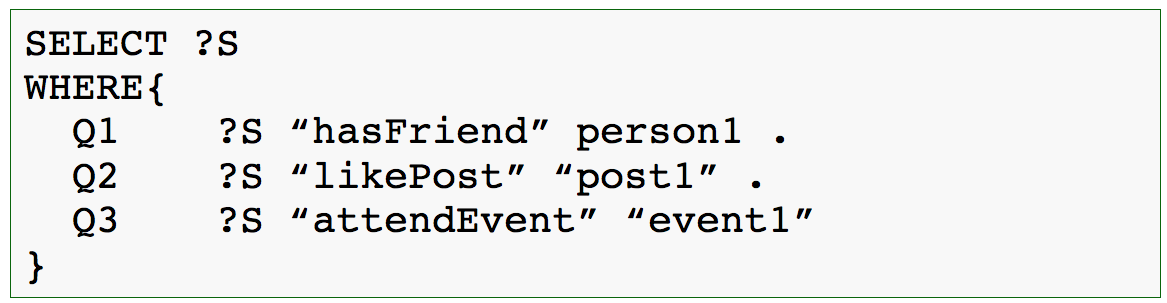
\includegraphics[width=0.5\textwidth]{figs/examplequery.png}
\end{center}
\vspace{-0.2in}
    \begin{center}
    	\includegraphics<1>[width=0.8\textwidth]{figs/implementation1.png}
    	\includegraphics<2>[width=0.8\textwidth]{figs/implementation2.png}
    \end{center}
\end{frame}


\begin{frame}
\frametitle{Outline}
	\begin{itemize}
		\item Introduction
		\item Query Decomposition and Data Partition
		\item Parallel and Distributed Query Planner
		\item Continuous Join
		\item Implementation
		\item Experiment Result
		\item \textcolor{blue!20}{Conclusion}
	\end{itemize}
\end{frame}

\begin{frame}
\frametitle{Experiment Setting}
\begin{itemize}
\item We evaluate the system on Grid 5000, with 11 nodes. 1 Master (Nimbus), 10 Slaves (Supervisor). 

\item The Storm version is 1.0, and we only use one slot on each machine.

\item Apache Jena API is used for reading triples.
\end{itemize}

\begin{itemize}
\item Synthetic data
\begin{itemize}
\item The RDF triples generated in Spouts are distributed to the nodes according to their predicate. 
\end{itemize}
\end{itemize}

\end{frame}


\begin{comment}
\begin{frame}
\frametitle{Evaluations}
\textbf{Impacts: (x axis)}
\begin{itemize}
\item Sliding Window Size
\item Number of Generations
\end{itemize}
\textbf{Metrics: (y axis)}
\begin{itemize}
\item Execution Latency --- The difference between the time an element is generated and the time it is emitted as a result
\item Process Latency --- The difference between the time an element is generated and the time it begins to be processed
\item Data Transmitted
\item Accuracy
\end{itemize}
\end{frame}
\end{comment}

\begin{frame}
\frametitle{Execution Lateny}
\vspace{-0.1in}
Sliding Window Size = 800 (1-Variable Join)    
    \begin{columns}
\begin{column}{0.45\textwidth}
More Generations $\Rightarrow$ More frequent updates $\Rightarrow$ Faster
\end{column}
\begin{column}{0.55\textwidth}
 		\includegraphics<1>[width=1.1\textwidth]{figs/II_1V_EL.png}
\end{column}
\end{columns} 
\end{frame}

\begin{frame}
\frametitle{Execution Latency}
\begin{columns}
\begin{column}{0.5\textwidth}
2-Variable Join
 	\includegraphics<1>[width=1.2\textwidth]{figs/II_2V_EL.png}
\end{column}
\begin{column}{0.5\textwidth}
Multiple-Variable Join
 	\includegraphics<1>[width=1.2\textwidth]{figs/II_MV_EL.png}
\end{column}
\end{columns}
\end{frame}


\begin{comment}
\begin{frame}
\frametitle{Execution Latency}
\vspace{-0.1in}
Number of Generation = 6 (1V)
\vspace{-0.2in}
\begin{center}
    	\includegraphics<1>[width=0.7\textwidth]{figs/III_1V_EL.png}
\end{center}
\end{frame}
\end{comment}


\begin{comment}
\begin{frame}
\frametitle{Processing Lateny}
\vspace{-0.1in}
Sliding Window Size = 800 (1V)
\vspace{-0.2in}
    \begin{center}
    	\includegraphics<1>[width=0.7\textwidth]{figs/II_1V_PL.png}
    \end{center}
\end{frame}


\begin{frame}
\frametitle{Processing Latency}
\vspace{-0.1in}
Number of Generation = 6 (1V)
\vspace{-0.2in}
\begin{center}
    	\includegraphics<1>[width=0.7\textwidth]{figs/III_1V_PL.png}
\end{center}
\end{frame}
\end{comment}

\begin{frame}
\frametitle{Data Transmitted -- Sliding Window Size = 800}
\textbf{Multiple-Variable Join}
\vspace{-0.2in}
\begin{center}
\includegraphics<1>[width=0.8\textwidth]{figs/II_MV_DT.png}
\end{center}

\end{frame}

\begin{frame}
\frametitle{Accuracy}
\textbf{We got 100\% correct results --- Surprise!}

Large Bloom Filters but very few matching elements.

%Because we use p and n to decide m. Each time n is set to the number of elements contained by each generation, but actually, the real number of elements inserted into the Bloom Filter should be the number of results which match the triple pattern, which is much less then what we set. Since each time we set p to 0.05\%, which is rather small, we didn't get any false positive results in our experiments.
\end{frame}

\begin{frame}
\frametitle{Outline}
	\begin{itemize}
		\item Introduction
		\item Query Decomposition and Data Partition
		\item Parallel and Distributed Query Planner
		\item Continuous Join
		\item Implementation
		\item Experiment Result
		\item Conclusion
	\end{itemize}
\end{frame}

\begin{frame}
\frametitle{Conclusion}
\begin{itemize}
\item Parallel and distributed join processing on RDF streams
\item Distribute both data and queries
\item Efficient
\begin{itemize}
\item Time 
\begin{itemize}
\item Execution Latency less than 600 ms
\end{itemize}
\item Space --- 400 times more efficient than without using Bloom FIlters
\end{itemize}
\end{itemize}
\end{frame}

\begin{comment}
\begin{frame}
\frametitle{Conclusion}
\vspace{-0.1in}
	\begin{itemize}
		\item Query Decomposition and Data Partition
		\begin{itemize}
		\item[-] According to predicate
		\end{itemize}
		\item Parallel and Distributed Query Planner
		\begin{itemize}
		\item[-] use Bloom Filter to communicate among sub-queries
		\item[-] 3 types of different kinds of joins according to the structure
		\item[-] one rule for communication order
		\end{itemize}
		\item Continuous Join
		\begin{itemize}
		\item[-] Sliding Window + Sliding Bloom Filter
		\end{itemize}
		\item Analysis
		\begin{itemize}
		\item[-] Bloom Filters
		\item[-] Dominating Parameters for the System
		\end{itemize}
		\item Implementation
		\begin{itemize}
		\item[-] Spout + BuilderBolt + ProberBolt
		\end{itemize}
		\item Experiment Result
		\begin{itemize}
		\item[-] Processing Latency + Execution Latency + Data Transmission
		\end{itemize}
	\end{itemize}
\end{frame}
\end{comment}